\documentclass[11pt,a4paper]{article}
\usepackage[T1]{fontenc}
\usepackage{lmodern}
\usepackage[margin=1in]{geometry}
\usepackage{amsmath,amssymb,array,longtable,tabularx,graphicx}
\usepackage[hidelinks]{hyperref}
\IfFileExists{microtype.sty}{\usepackage{microtype}}{}
\linespread{1.07}
\setlength{\parskip}{0.5em}
\setlength{\parindent}{0pt}
\setlength{\emergencystretch}{3em}
\renewcommand{\topfraction}{0.95}
\renewcommand{\bottomfraction}{0.9}
\renewcommand{\textfraction}{0.05}
\renewcommand{\floatpagefraction}{0.85}
\setcounter{topnumber}{4}
\setcounter{totalnumber}{6}
\renewcommand{\arraystretch}{1.18}
\newcommand{\toprule}{\hline\noalign{\smallskip}}
\newcommand{\midrule}{\noalign{\smallskip}\hline\noalign{\smallskip}}
\newcommand{\bottomrule}{\noalign{\smallskip}\hline}
\newcommand{\op}[1]{\texttt{#1}}
\newcommand{\AIG}{\mathrm{AIG}}
\makeatletter
\setlength{\@fptop}{0pt}
\setlength{\@fpsep}{18pt}
\setlength{\@fpbot}{0pt plus 1fil}
\renewcommand\section{\@startsection{section}{1}{\z@}{1.3em}{.4em}{\normalfont\large\bfseries}}
\renewcommand\subsection{\@startsection{subsection}{2}{\z@}{1em}{.3em}{\normalfont\normalsize\bfseries}}
\newenvironment{inlinefigure}{\par\addvspace{12pt}\noindent\begin{minipage}{\textwidth}\def\@captype{figure}\centering}{\end{minipage}\par\addvspace{12pt}}
\makeatother
\newcommand{\MaxNodes}{27,062}
\newcommand{\SuccessfulRuns}{24,600}
\newcommand{\ProbeSeconds}{0.91}
\newcommand{\SweepMinutes}{30.7}
\newcommand{\MedianNodes}{327}
\newcommand{\MedianDepth}{16}
\newcommand{\MeanArea}{0.834}
\newcommand{\MeanDelay}{0.875}
\newcommand{\DistinctWinners}{85}
\newcommand{\OracleGain}{9.15\%}
\newcommand{\PrimaryGain}{0.73\%}
\newcommand{\PrimaryCI}{[0.25\%, 1.18\%]}
\newcommand{\PrimaryRegret}{9.01\%}
\newcommand{\PrimaryP}{2.82\times10^{-4}}
\newcommand{\GlobalEightRegret}{3.00\%}
\newcommand{\GlobalEightSeconds}{3.18}
\newcommand{\LearnedFiveRegret}{3.95\%}
\newcommand{\LearnedFiveSeconds}{3.11}

\newcommand{\NNGain}{0.19\%}
\newcommand{\NNCI}{[-0.40\%, 0.79\%]}
\newcommand{\NNRegret}{9.60\%}
\newcommand{\NNStaticGain}{0.44\%}
\newcommand{\NNFiveGain}{5.12\%}
\newcommand{\NNFiveRegret}{3.99\%}
\newcommand{\NNOneSeconds}{1.39}
\newcommand{\NNFiveSeconds}{2.92}
\newcommand{\ExhaustiveSeconds}{44.84}
\newcommand{\NNOneSpeedup}{32.2}
\newcommand{\NNFiveSpeedup}{15.4}
\newcommand{\NNOneSaved}{96.89\%}
\newcommand{\NNFiveSaved}{93.49\%}


\title{\textbf{Neural Recipe Selection for Logic Synthesis\\Quality and Compute on Unseen Circuits}}
\author{Shaan Chopra (240905140), Kenneth Rodrigues (240905112),\\
Darren Pais (240905093), and Aniket Verma (240905156)\\[0.4em]
\small School of Computer Science and Engineering\\
\small Manipal Institute of Technology}
\date{October 2026}

\begin{document}
\maketitle
\begin{abstract}
\noindent
Logic synthesis applies sequences of transformations to reduce a digital circuit's area and delay. Finding a good sequence by trying every candidate repeats substantial computation for each new circuit. We train a small neural network to recommend sequences from a fixed library of 120 recipes. Training uses 24,600 measured outcomes from 205 public benchmark circuits, generated with ABC and a NanGate 45\,nm cell library. The network receives circuit features and predicts all recipe scores in one pass. On unseen circuits in repeated nested cross-validation, one recommendation gives \NNGain\ mean improvement over the best fixed training recipe, with a 95\% interval of \NNCI. Five recommended recipes give \NNFiveGain\ improvement and \NNFiveRegret\ mean regret relative to the best of all 120 recipes. In a separate serial timing audit on 12 circuits, these one- and five-recipe choices take \NNOneSeconds\,s and \NNFiveSeconds\,s, including feature collection, compared with \ExhaustiveSeconds\,s for exhaustive search: \NNOneSpeedup-fold and \NNFiveSpeedup-fold speedups. A global shortlist achieves similar quality with less selection overhead. The results quantify the quality--compute trade-off and provide a trained selector for new circuits.
\end{abstract}

\section{Introduction}

A digital circuit computes a function of binary inputs. An adder, for example, receives two binary numbers and produces their sum. Many different networks of logic gates can compute the same function. Their physical implementations can occupy different amounts of chip area and take different amounts of time to produce an output.

\emph{Logic synthesis} searches for a useful implementation of that function. A synthesis tool can simplify expressions, share repeated computations, and restructure long chains of gates. These transformations preserve the function. Their order matters because one transformation changes the opportunities available to the next. A sequence of transformations is called a \emph{recipe}.

Engineers often begin with a standard recipe that works reasonably well across designs. Another approach tries many recipes separately on each circuit. We study whether machine learning can use experience from earlier circuits to choose a useful recipe for a new one. The practical objective is to obtain a good implementation after a small number of complete synthesis runs.

We build a table of measured outcomes for 205 circuits and 120 recipes, then train a neural network to recommend recipes for a circuit it has never seen. The expensive table is collected once during development. For a new circuit, the network uses features available before recipe execution, predicts 120 scores, and recommends either one recipe or a short list. Only those recommended recipes are synthesized.

We compare the resulting area--delay objective with two central references. The \emph{best fixed recipe} is the single recipe with the lowest mean training objective; it is reused on every new circuit. The \emph{exhaustive-search oracle} tries all 120 recipes on each circuit and keeps its best result. Our question is how much computation a learned recommendation saves, and how much quality it retains. We also compare with globally ranked shortlists and classical supervised models to assess the value of adapting the recommendation to each circuit.

\begin{inlinefigure}
\centering
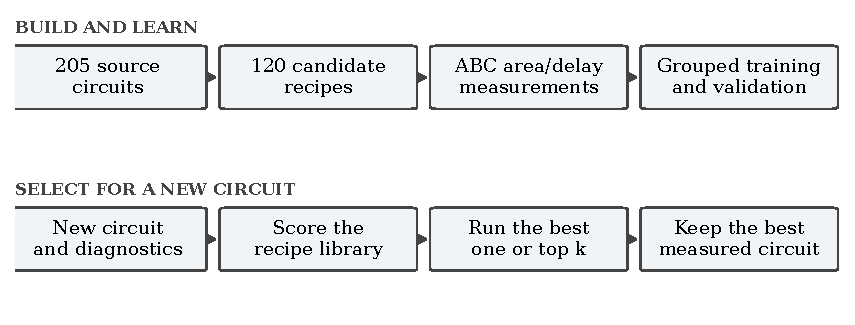
\includegraphics[width=\textwidth]{figures/workflow.pdf}
\caption{The experiment has a dataset-building stage and a selection stage. During evaluation, the new circuit belongs to an outer test fold and contributes no labels to training or tuning.}
\label{fig:workflow}
\end{inlinefigure}

\section{Circuit Concepts and the Synthesis Process}
\label{sec:background}

\subsection{Combinational circuits, area, and delay}

Our circuits are \emph{combinational}: their outputs depend on their current inputs. They contain no memory elements such as registers or latches. This gives each circuit a fixed Boolean input--output function.

\emph{Area} is the sum of the areas of the logic cells used to implement the circuit, measured here in square micrometres ($\mu\mathrm{m}^2$). Lower area allows the logic to occupy less chip space. \emph{Delay} is the estimated time along the slowest input-to-output path, measured in picoseconds (ps). Lower delay allows an output to become valid sooner and can help a design meet its timing requirement. Area and delay can trade off: a larger cell may drive a signal faster, while sharing logic can reduce area and add a longer path.

ABC estimates these quantities after \emph{technology mapping}: assigning the logic to small predesigned gates, called standard cells, from a technology library. The library is a catalogue of available cell functions, areas, and timing models. We use the NanGate Open Cell Library for a nominal 45\,nm technology at its typical operating corner, meaning its nominal voltage and temperature condition~\cite{nangate}. The resulting \emph{netlist} lists the cells and their connections. Our measurements come from synthesis and cell timing with no wire-load model. Placement and routing would add physical interconnect effects.

\subsection{And-Inverter Graphs}

ABC represents the circuit internally as an \emph{And-Inverter Graph} (AIG)~\cite{abc,mishchenko}. Each internal node computes AND of two signals; an edge can invert its signal. This representation can express arbitrary Boolean logic. For example, OR can be expressed using AND and inversion:
\[
a\lor b=\neg(\neg a\land\neg b).
\]
Input nodes supply signals, output connections identify the results, and shared graph nodes represent shared computations. The graph is directed and has no cycles for a combinational circuit.

Two simple graph measurements are the number of AND nodes and the number of \emph{levels}: the largest number of AND nodes on an input-to-output path. Node count summarizes logic size; levels summarize logical depth. They are useful structural features. The final cell area and timing also depend on how groups of nodes map to the library's cells.

ABC's \op{strash} command constructs a structurally hashed AIG, merging identical AND nodes. We use this graph as the starting point for every recipe on a circuit.

\subsection{What a recipe does}
\label{sec:ops}

Our vocabulary contains seven operations, listed in Table~\ref{tab:operations}. Each operation visits and transforms the current graph. A recipe applies its operations sequentially to that graph. The next operation therefore receives the previous operation's result.

\begin{table}[htbp]
\centering\small
\begin{tabularx}{\textwidth}{@{}p{1.8cm}p{2.8cm}X@{}}
\toprule
\textbf{Symbol} & \textbf{ABC command} & \textbf{Purpose}\\
\midrule
\op{rw}, \op{rwz} & \op{rewrite}, \op{rewrite -z} & Replace small parts of the graph with equivalent structures, using existing shared logic where possible.\\
\op{rf}, \op{rfz} & \op{refactor}, \op{refactor -z} & Re-express a larger logic region through factoring. For example, repeated terms in $ab+ac$ suggest the factored form $a(b+c)$.\\
\op{rs}, \op{rsz} & \op{resub}, \op{resub -z} & Express a function using signals already computed elsewhere in the circuit.\\
\op{b} & \op{balance} & Restructure chains of associative logic into a shallower arrangement.\\
\bottomrule
\end{tabularx}
\caption{Recipe operations. The \op{-z} variants also allow replacements with no immediate reduction in graph size. Such a replacement can create opportunities for a later operation. It still takes computation time.}
\label{tab:operations}
\end{table}

The standard recipe \op{resyn2} interleaves ten passes~\cite{mishchenko}:
\begin{center}
\op{b rw rf b rw rwz b rfz rwz b}.
\end{center}
For example, it first balances the graph, then rewrites it, then refactors it. We include this explicit sequence as recipe R001 and use it as a reference throughout the experiment. The model selects a complete sequence from the candidate library.

\par\noindent\begin{minipage}{\textwidth}
\subsection{One complete measurement}
\label{sec:measurement}

For each circuit--recipe pair, we start a fresh ABC process and execute:
\par
\begin{verbatim}
read_lib -w NangateOpenCellLibrary_typical.lib
read_blif circuit.blif       # read_bench for a .bench input
strash
balance; rewrite; ...       # all operations in one recipe
print_stats
map
topo
stime
\end{verbatim}
\end{minipage}
\par

The input file describes a network of Boolean logic. BLIF and BENCH are text formats that ABC can read directly. After the recipe finishes, \op{map} assigns the resulting logic to cells from the library. The \op{topo} command orders the mapped network for timing analysis, and \op{stime} reports area and delay. We map once, after the complete recipe.

Every candidate recipe starts again from the original circuit and its hashed AIG. Recipe R002 therefore does not inherit the graph produced by R001. The baseline measurement follows the same process with the recipe line omitted. This gives each circuit its own baseline area $A_0$ and delay $D_0$.

\section{Dataset Construction}
\label{sec:dataset}

\subsection{Circuit sources and inventory}

We retain the 205-circuit inventory from our pilot study. We retrieve EPFL inputs from the EPFL benchmark repository~\cite{epfl}; ISCAS-85 and MCNC inputs come from the ISP RAS \op{hdl-benchmarks} repository~\cite{hdl}. MCNC and LGSynth'91 originate from the 1991 logic-synthesis benchmark collections. Our selected files are from the MCNC combinational BLIF directory. The distribution is shown in Table~\ref{tab:pool}.

\begin{table}[htbp]
\centering\small
\begin{tabular}{@{}lrrrrr@{}}
\toprule
\textbf{Family} & \textbf{Circuits} & \textbf{Min. nodes} & \textbf{Median} & \textbf{Max. nodes} & \textbf{Depth median} \\
\midrule
EPFL arithmetic & 7 & 1,020 & 5,416 & 27,062 & 255 \\
EPFL control & 9 & 174 & 693 & 13,758 & 20 \\
ISCAS-85 & 10 & 209 & 610 & 2,337 & 30 \\
MCNC & 179 & 40 & 270 & 7,803 & 14 \\
\bottomrule
\end{tabular}

\caption{Circuit inventory. Size and depth refer to the starting hashed AIG. The four families are also used for validation across circuit types.}
\label{tab:pool}
\end{table}

EPFL contains arithmetic designs such as adders and multipliers, together with controllers, encoders, and related logic. ISCAS-85 provides established gate-level test circuits. MCNC contributes many smaller logic networks and supplies most of the independent training examples.

The pilot inventory retains circuits with no latches, at least four primary inputs, and at least 40 AND nodes. Its size limits are 30,000 AND nodes for EPFL and 8,000 for MCNC. ISCAS-85 circuits fit below 2,400 nodes. The inventory excludes the ISCAS-85 copies distributed inside MCNC and removes three duplicate signatures based on input count, output count, node count, and depth. These four counts are a coarse screening signature; different functions can share them. We retain the resulting inventory consistently across our experiments and save a source-file checksum for every circuit.

There are 179 MCNC circuits and 26 circuits from the other three families. We therefore report family-specific results and explicitly test transfer between families. The largest circuit has \MaxNodes\ AND nodes. The inventory concentrates on benchmark-scale combinational logic.

\subsection{The 120-recipe library}

Each recipe contains 6--12 operations. We preserve the pilot's 60 sequences and add 60 new sequences with random seed 17. The final library contains two established scripts, \op{resyn} and \op{resyn2}, plus 24 area-weighted, 24 delay-weighted, 24 mixed, and 46 uniformly sampled recipes.

The labels describe sampling distributions. Area-weighted sampling favors rewriting, refactoring, and resubstitution; delay-weighted sampling favors balancing. Mixed sampling gives balancing a modest extra weight. Length is sampled uniformly, duplicate sequences are rejected, and consecutive balancing operations are rejected. Each sequence is evaluated to establish its actual performance. Its sampling label is excluded from the model inputs.

\subsection{Labels and objective}

The completed dataset contains one row for each of the $205\times120=24,600$ circuit--recipe experiments. Each row stores the circuit family and identifier, starting-circuit features, recipe operations, baseline measurements, post-recipe measurements, and runtime. All \SuccessfulRuns\ runs completed successfully. The same 120 candidates are available for every circuit.

We normalize the mapped measurements by that circuit's baseline:
\begin{equation}
y_A(C,R)=\frac{A(C,R)}{A_0(C)},\qquad
y_D(C,R)=\frac{D(C,R)}{D_0(C)}.
\end{equation}
A value of 0.90 means a 10\% reduction from the corresponding baseline. This normalization lets us compare improvements across circuits of different sizes.

We combine the two outcomes using a weight $\lambda$:
\begin{equation}
J_\lambda(C,R)=\lambda y_A(C,R)+(1-\lambda)y_D(C,R).
\label{eq:objective}
\end{equation}
Lower is better. Our primary experiment uses $\lambda=0.5$, giving equal weight to relative area and delay. Separate experiments use $\lambda=0$ for delay and $\lambda=1$ for area. A score of 0.90 is a 10\% reduction in this weighted normalized objective; the individual area and delay changes are reported separately when interpreting a selected implementation.

\begin{table}[htbp]
\centering\small
\begin{tabular}{@{}lrrrrr@{}}
\toprule
\textbf{Recipe} & \textbf{Area ($\mu$m$^2$)} & \textbf{Delay (ps)} & \textbf{$y_A$} & \textbf{$y_D$} & \textbf{$J_{0.5}$} \\
\midrule
R001 (resyn2) & 385.97 & 621.87 & 1.083 & 0.929 & 1.006 \\
R037 & 343.94 & 602.63 & 0.965 & 0.900 & 0.932 \\
\bottomrule
\end{tabular}

\caption{Two measured recipes for circuit \op{c1908}. Its baseline area is 356.44\,$\mu\mathrm{m}^2$ and baseline delay is 669.63\,ps. R037 gives lower area and delay than \op{resyn2} on this circuit.}
\label{tab:example}
\end{table}

\section{Features and Learning}
\label{sec:learning}

\subsection{Describing the circuit}

We extract 50 circuit features in three groups. Their definitions and reasons for inclusion are summarized below; Appendix~\ref{app:features} gives the complete structural list.

\textbf{Static graph statistics (24).} Input and output counts describe the interface. Node count and depth describe size and path length. \emph{Fanout}, the number of connections using a signal, describes sharing and branching. The number of nodes at each level describes whether the graph is wide or concentrated along long paths. Differences between the levels of an AND node's two inputs indicate uneven paths that balancing may change. Additional statistics measure complemented edges, small exclusive-OR patterns, and nearby paths that split and meet again. We parse these quantities from ABC's binary AIGER graph export. We apply $\log(1+x)$ to ten size-like features so that large circuits have a more moderate numerical scale.

\textbf{Mapping baseline features (4).} We add $\log A_0$, $\log D_0$, area per AND node, and delay per graph level. These measurements describe how the starting graph maps to the chosen cell library. They are available before a candidate recipe is selected.

\textbf{Probe responses (22).} A probe is a short diagnostic transformation. Starting from the original hashed graph, we apply each of the seven operations once and record the ratios of its resulting node count and depth to the starting values. This gives 14 features. We also apply four two-step probes: \op{b rw}, \op{rw b}, \op{rf b}, and \op{b rf}. Their node and depth ratios give eight more features. These pairs expose order sensitivity. Each probe starts independently from the same graph; probes never accumulate into a longer optimization chain. They stop before mapping, so their outputs are graph measurements. The complete probe set takes \ProbeSeconds\ seconds per circuit on average in our sweep environment.

\subsection{Describing the recipe}

The neural network has one output for each of the 120 known recipes. An output's position identifies its recipe, so the network needs only circuit features as input. The saved model includes the mapping from outputs to complete operation sequences. This formulation assumes that the candidate library stays fixed; adding recipes requires new output labels and a refitted model.

For the classical circuit--recipe regressors, we also construct a 144-feature recipe encoding: length and count of \op{-z} operations (2), counts of the seven operations (7), one-hot operation identities at 12 positions (84), counts of the 49 ordered adjacent operation pairs, and indicators for a balancing operation at the beginning and end (2). Short sequences use zero padding at unused positions.

Operation counts describe the mixture of transformations. Position and transition features preserve order: \op{rw b} and \op{b rw} have identical operation counts but different position and transition values. The classical models' full circuit--recipe input has $50+144=194$ features. Circuit identifiers, measured post-recipe area and delay, post-recipe graph statistics, and runtimes are excluded from predictors.

\subsection{Predicting relative performance}

The selector needs a useful ordering of recipes for the same circuit. Some circuits improve substantially under almost any recipe; others offer little improvement. To focus the model on differences between recipes, we center the training objective within each training circuit:
\begin{equation}
\widetilde J(C,R)=J(C,R)-\frac{1}{|\mathcal R_{\mathrm{train}}|}
\sum_{R'\in\mathcal R_{\mathrm{train}}}J(C,R').
\end{equation}
A negative target means that a recipe is better than that circuit's average candidate. At prediction time, the model ranks recipes using the predicted centered values. All candidates for a circuit share the same missing offset, so this ranking requires no test-circuit outcome labels.

\subsection{The neural network}

Our main network is a multilayer perceptron (MLP) with 50 inputs, hidden layers of 64 and 32 units, and 120 linear outputs: 9,304 trainable parameters. ReLU activations allow nonlinear relationships between circuit features and recipe outcomes. Dropout with probability 0.1 regularizes the hidden layers during training. We also evaluate an otherwise identical network with the 24 static graph features as its input. This variant skips mapping-derived inputs and diagnostic probes.

Each training example is one circuit with its vector of 120 centered outcomes. For each recipe, we compute its mean centered training outcome $\mu_R$. The network learns the remaining circuit-specific adjustment:
\begin{equation}
\widehat{\widetilde J}(C,R)=\mu_R+s\,f_\theta(x_C)_R.
\end{equation}
Here $x_C$ is the standardized circuit feature vector, $f_\theta$ is the MLP, and $s$ is the standard deviation of the training residuals $\widetilde J(C,R)-\mu_R$, pooled across circuits and recipes. Subtracting $\mu_R$ and dividing by $s$ gives the regression targets used in training. We standardize input features using training-circuit means and standard deviations. Every statistic is recomputed inside its training partition.

We initialize the final layer to zero. The initial prediction therefore ranks recipes by their training means, which gives the best fixed recipe. Training learns how to adjust that ranking for each circuit. We minimize mean squared error across all training circuits and recipe outputs using full-batch AdamW. The learning rate is 0.003 and weight decay is 0.03. Three-fold inner validation chooses 25, 75, or 200 training epochs. The selected network is then refitted on the outer training circuits. At inference, dropout is disabled and all 120 scores are produced in one forward pass.

\subsection{Classical model comparisons}

We compare five additional model variants: additive ridge regression, ridge with explicit interactions, Extra-Trees, Random Forest, and gradient-boosted decision trees implemented with LightGBM. The interaction ridge model multiplies each of the 22 probe features by each of the seven operation counts, adding 154 columns. The ordinary ridge model adds separate circuit and recipe contributions. Its predicted recipe ordering is therefore the same for every circuit. The interaction features allow its ordering to depend on the circuit; the tree models learn interactions through their splits.

We standardize features for ridge using statistics fitted on the training partition. We also compare raw $J$ targets and within-circuit ranks scaled to $[0,1]$ in the target ablation. Every target transformation uses only the training rows available to that fit.

\subsection{Turning predictions into a decision}

The neural selector chooses the recipe with the lowest predicted score. A recommendation is a complete operation sequence, applied once from the original hashed circuit as described in Section~\ref{sec:measurement}. We evaluate the two NN input variants separately. Our classical comparisons also include an \emph{adaptive selector} that chooses among the five classical model families and their settings using inner validation.

We also evaluate two extensions. A \emph{margin gate} uses the predicted best recipe when its predicted advantage over the best fixed recipe exceeds a threshold; otherwise it uses that fixed recipe. We tune the threshold inside the training partition. A \emph{top-$k$ selector} executes the $k$ lowest-scored recipes, measures their actual mapped outcomes, and keeps the best. We use $k\in\{1,2,3,5,8\}$. The shortlist ranking is determined entirely by the model; the final choice among those executed candidates uses their measurements.

\section{Validation and Comparisons}
\label{sec:validation}

\subsection{Unseen circuits and nested tuning}

The independent examples are the 205 circuits. The 24,600 rows contain repeated observations of those circuits. We keep every recipe row belonging to a circuit in the same partition.

Our primary protocol uses five circuit folds repeated three times with seeds 0, 1, and 2. Families are stratified where the available counts permit. In each outer fold, approximately 164 circuits are used for training and 41 are held out for testing. Every circuit is tested once per repeat.

Inside an outer training partition, three-fold circuit-grouped validation selects model settings. Its criterion is mean percentage improvement over the best fixed recipe learned from the corresponding inner training circuits. The NN uses exactly the same outer partitions and inner splitting seeds as the classical experiments. The classical adaptive selector also chooses its model family using these inner results. We then refit on the complete outer training partition and evaluate its recipe choices on the outer test circuits. This separates training, tuning, and testing at the circuit level. Table~\ref{tab:grid} gives the tuning grid.

The exhaustive dataset supplies the outcome of every candidate. We evaluate a selector by first making its feature-based decision and then looking up the measured outcome of its chosen recipe. A top-$k$ selector can use the measurements of its $k$ recommended candidates to choose its final result. The complete test-circuit outcome table is used to compute the evaluation metrics and oracle reference.

\begin{table}[htbp]
\centering\small
\begin{tabularx}{\textwidth}{@{}p{3.7cm}X@{}}
\toprule
\textbf{Model} & \textbf{Settings and inner-validation choices}\\
\midrule
Neural network & Hidden layers 64 and 32; dropout 0.1; AdamW learning rate 0.003, weight decay 0.03; epochs in $\{25,75,200\}$. Separate 50-input and 24-input evaluations.\\
Ridge, interaction ridge & Regularization $\alpha\in\{10,100\}$; training-fitted standardization.\\
Extra-Trees, Random Forest & 80 trees; maximum depth 16; 30\% of features considered per split; minimum leaf size in $\{5,15\}$.\\
LightGBM & 180 trees; learning rate 0.05; minimum leaf size 20; $L_2$ penalty 1; number of leaves in $\{15,31\}$.\\
Margin gate & Predicted advantage threshold in $\{0,0.0025,0.005,0.01,0.02\}$.\\
\bottomrule
\end{tabularx}
\caption{Model settings. Neural inputs describe one circuit and its outputs score the 120 recipes. Classical regressors use 194 circuit--recipe features; interaction ridge additionally uses 154 explicit products. All fits use training-only statistics.}
\label{tab:grid}
\end{table}

\subsection{Reference selectors}

\textbf{Best fixed recipe.} We average each recipe's measured objective across the training circuits and choose the smallest average. That single recipe is then used on every test circuit. We recompute it separately inside every training split. It is the primary comparator.

\textbf{\op{resyn2}.} We execute the standard ten-operation script described in Section~\ref{sec:ops}. This is a familiar synthesis reference and is distinct from the no-recipe normalization baseline.

\textbf{Random choice.} We report the expected result of uniform recipe selection. For a budget of $k$ runs, we compute the exact expected best outcome among $k$ distinct uniformly sampled recipes.

\textbf{Global top-$k$.} We execute the $k$ recipes with the best training-set mean objectives and keep their best measured result on each test circuit. This is the budget-matched comparator for a learned shortlist.

\textbf{Oracle.} We take the best measured recipe in the entire candidate library for each circuit. This summarizes the improvement available within the library. It requires the exhaustive measurements of all 120 recipes.

\subsection{Metrics, uncertainty, and execution cost}

For each test circuit, we compute percentage improvement over the fixed training recipe:
\begin{equation}
\mathrm{Improvement}(C)=100\,
\frac{J_{\mathrm{fixed}}(C)-J_{\mathrm{selected}}(C)}{J_{\mathrm{fixed}}(C)}.
\end{equation}
Positive values favor the selector. Our main NN comparison uses one recommendation from the 50-feature network at $\lambda=0.5$. We also report the 24-feature network, larger verification budgets, classical model comparisons, and regret relative to the oracle:
\begin{equation}
\mathrm{Regret}(C)=100\,
\frac{J_{\mathrm{selected}}(C)-J_{\mathrm{oracle}}(C)}{J_{\mathrm{oracle}}(C)}.
\end{equation}
Regret is zero when the selected outcome reaches the best measured library outcome. Spearman correlation measures within-circuit ranking quality; we assign zero when predictions or measured outcomes are constant within a circuit.

We average repeated-test improvements for each circuit, then bootstrap those 205 circuit averages with 2,000 resamples to obtain 95\% intervals. Each circuit receives equal weight. These intervals describe variation across the benchmark circuits under the saved validation procedure. A paired Wilcoxon signed-rank test additionally describes the classical adaptive comparison. A small mean difference and an interval covering zero establish uncertainty about the gain; formal equivalence would require a specified acceptable quality margin.

Execution cost includes graph extraction, baseline mapping, the probes used by the model, prediction, and all $k$ executed recipe runs. The graph-only NN skips probes; we still include a baseline mapping to report its normalized objective. For global shortlists with two or more candidates, baseline mapping supplies the normalization needed to compare their area--delay objectives. A single fixed recipe can be selected and executed without that measurement.

We measure runtime separately on 12 circuits: the nearest 25th-, 50th-, and 75th-percentile AIG sizes within each of the four source families. Selection uses the first repeat's saved outer-fold NN, which has never trained on that timing circuit. On each circuit, we run baseline mapping, feature extraction, and all 120 recipes serially. Every measured area and delay must reproduce the dataset. We then sum the feature, prediction, and selected-candidate times for each method. Exhaustive-search time includes baseline mapping and all 120 recipe runs. This compares methods using the same candidate timings and execution setting.

Prediction timing includes feature preprocessing with the model already loaded. We use the median of seven repeated predictions per timing circuit. Process startup and model loading are paid separately by an application that launches the predictor anew; the supplied command reports model-load time separately. Runtime-audit quality refers to those 12 circuits. The main quality estimates continue to use all 205 circuits and all three repeats.

\subsection{Transfer, ablations, and unseen sequences}

We train on the 179 MCNC circuits and test on the 26 EPFL and ISCAS-85 circuits to examine transfer to a different mixture of designs. We also hold out each of the four families in turn.

The feature ablation compares static graph statistics, static plus mapping measurements, all features, and probes alone. The recipe-encoding ablation adds positions and then transitions to operation counts. Target ablations compare raw, centered, and ranked objectives. Library experiments use 30, 60, and 120 candidates. We use the boosting model and one five-fold repeat for these controlled comparisons, tuning its settings inside each training fold. The 60-recipe experiment uses the original pilot library; the 30-recipe subset retains both established scripts and samples the other strata with a fixed seed.

We also repeat the boosting experiment with 25, 50, and 100 randomly sampled training circuits per outer fold. The outer test circuits stay fixed, and the same circuit-count limit applies before inner tuning. This measures how selection quality changes with the number of independent training designs.

For the unseen-recipe experiment, we reserve 24 sequences, stratified across the sampled recipe groups. Their labels are removed from all training and inner-validation partitions. On held-out circuits, the model scores the full 120-recipe library, including the reserved sequences. This tests whether the sequence encoding supports selection when some candidate recipes have no training labels. Both established scripts remain available during training.

\section{Results}
\label{sec:results}

\subsection{Measured dataset and selection headroom}

The full sweep completed in \SweepMinutes\ minutes using five synthesis workers. The median circuit has \MedianNodes\ AND nodes and depth \MedianDepth. Across all measured pairs, the mean normalized area is \MeanArea\ and the mean normalized delay is \MeanDelay. These dataset averages summarize the candidate library's behavior before learning.

The best recipe varies across circuits. With ties resolved by recipe identifier, the oracle selects \DistinctWinners\ different sequences across the pool at $\lambda=0.5$. Selecting each circuit's best measured recipe gives \OracleGain\ mean improvement over the leave-one-circuit-out best fixed recipe. This establishes the library's circuit-specific selection headroom.

\begin{inlinefigure}
\centering
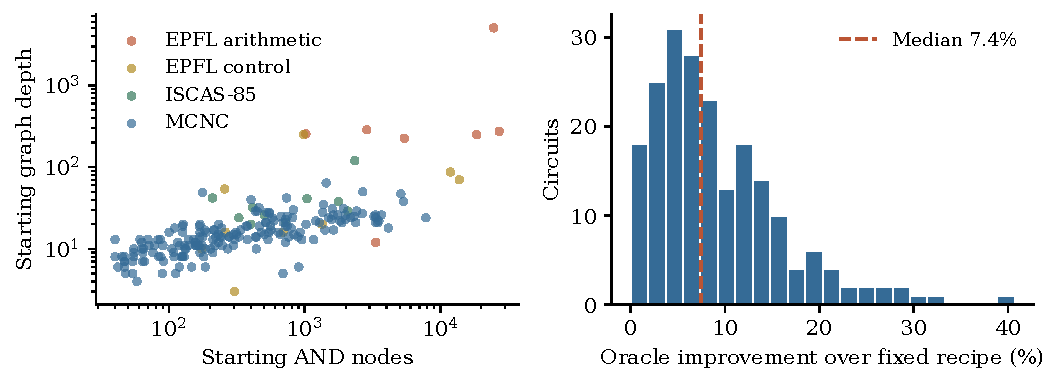
\includegraphics[width=\textwidth]{figures/dataset.pdf}
\caption{Circuit pool and available selection headroom. Left: starting AIG size and depth, colored by source family. Right: improvement of each circuit's best measured recipe over a fixed recipe chosen from the other 204 circuits, at $\lambda=0.5$.}
\label{fig:dataset}
\end{inlinefigure}

\subsection{Neural recommendations on held-out circuits}

Table~\ref{tab:nn-quality} compares neural recommendations with the fixed recipe, a global shortlist, and exhaustive search. A one-recipe selector commits to its prediction. A five-recipe selector executes only its five recommendations and keeps the best measured result. Exhaustive search executes all 120 candidates.

\begin{table}[htbp]
\centering\small
\begin{tabular}{@{}lrrrr@{}}
\toprule
\textbf{Selector} & \textbf{Runs} & \textbf{Gain (\%)} & \textbf{95\% interval} & \textbf{Regret (\%)} \\
\midrule
NN, 50 circuit features & 1 & 0.19 & [-0.40, 0.79] & 9.60 \\
NN, 24 graph features & 1 & 0.44 & [-0.28, 1.10] & 9.25 \\
NN, 50 features; top five & 5 & 5.12 & [4.54, 5.70] & 3.99 \\
NN, 24 features; top five & 5 & 4.80 & [4.21, 5.39] & 4.35 \\
Global top five & 5 & 5.01 & [4.50, 5.55] & 4.13 \\
Best fixed recipe & 1 & 0.00 & [0.00, 0.00] & 9.97 \\
Exhaustive search & 120 & 8.61 & [7.90, 9.39] & 0.00 \\
\bottomrule
\end{tabular}

\caption{Quality on all 205 circuits using three repeats of nested five-fold validation. Gain is the percentage reduction in the normalized area--delay objective relative to the best fixed training recipe. Oracle regret is the remaining percentage gap to the best of 120 recipes.}
\label{tab:nn-quality}
\end{table}

With one complete recipe execution, the 50-feature network gave 0.19\% mean improvement over the best fixed training recipe, with a 95\% interval of [-0.40\%, 0.79\%]. The 24-feature network gave 0.44\% with interval [-0.28\%, 1.10\%]. Both point estimates are close to the fixed-recipe result; the intervals include zero, leaving the direction of the average difference uncertain. For the 50-feature network, mean area fell by 0.31\% and mean delay rose by 0.47\% relative to the fixed recipe.

Running the full network's five highest-ranked recipes gave 5.12\% improvement over the fixed recipe and 3.99\% mean oracle regret. It reached the exact library optimum on 15.28\% of held-out predictions and came within 5\% of it on 70.24\%. These rates average the three held-out predictions per circuit. The corresponding mean area and delay reductions were 2.44\% and 7.17\%.

The global top-five baseline improved the fixed-recipe objective by 5.01\% with 4.13\% regret. The NN top-five result improved this global shortlist by 0.06\% on average (95\% interval [-0.36\%, 0.48\%]). This interval also includes zero. The experiments show how a small candidate budget recovers much of the available quality; the global shortlist remains a strong inexpensive alternative.


\subsection{Compute saved on a new circuit}

Table~\ref{tab:nn-runtime} reports the serial timing audit. Each circuit is unseen by the saved model used for its recommendation. The candidate timings come from fresh executions of all 120 recipes on that circuit, allowing a direct comparison of search budgets. All 1,440 outcomes reproduced their dataset area and delay.

\begin{table}[htbp]
\centering\small
\begin{tabular}{@{}lrrrr@{}}
\toprule
\textbf{Selector} & \textbf{Runs} & \textbf{Time (s)} & \textbf{Speedup ($\times$)} & \textbf{Saved (\%)} \\
\midrule
Best fixed recipe & 1 & 0.406 & 110.4 & 99.1 \\
NN, 50 features & 1 & 1.393 & 32.2 & 96.9 \\
NN, 24 features & 1 & 0.773 & 58.0 & 98.3 \\
Global top five & 5 & 2.221 & 20.2 & 95.0 \\
NN, 50 features; top five & 5 & 2.917 & 15.4 & 93.5 \\
NN, 24 features; top five & 5 & 2.312 & 19.4 & 94.8 \\
Global top eight & 8 & 3.410 & 13.1 & 92.4 \\
Exhaustive search & 120 & 44.839 & 1.0 & 0.0 \\
\bottomrule
\end{tabular}

\caption{Mean serial time over 12 size-stratified circuits, including feature collection and executed recipes. Speedup is the ratio of mean exhaustive time to mean selector time; saved time is its corresponding percentage reduction. Models are already loaded.}
\label{tab:nn-runtime}
\end{table}

Across the 12 timing circuits, exhaustive search took 44.84 seconds per circuit on average. One full-network recommendation, including diagnostics and its synthesis run, took 1.39 seconds: 32.2 times faster and 96.89\% less elapsed time. Executing five recommendations took 2.92 seconds, giving a 15.4-fold speedup and 93.49\% time saving. The graph-only network with one executed recipe took 0.77 seconds (58.0-fold speedup).

The global top-five baseline took 2.22 seconds. It avoids the eleven diagnostic probes and also reduces exhaustive-search cost substantially. Table~\ref{tab:nn-runtime} therefore separates the savings from executing fewer candidates from the additional cost of neural selection. The speedups divide mean exhaustive time by mean selector time on the same 12 circuits. They describe serial execution with a loaded model; parallel exhaustive search would have a different elapsed-time trade-off.

The training table was built once in 30.7 minutes with five ABC workers. The complete NN evaluation, including both input variants, three repeats, and inner tuning, took 90.7 seconds. Refitting the full network after settings were chosen took 0.100 seconds per outer fold on average. These are development costs. A new circuit uses the saved model and pays only feature collection, prediction, and its chosen recipe runs. The measured search table is shared by the fixed-recipe baseline and the NN.


\begin{inlinefigure}
\centering
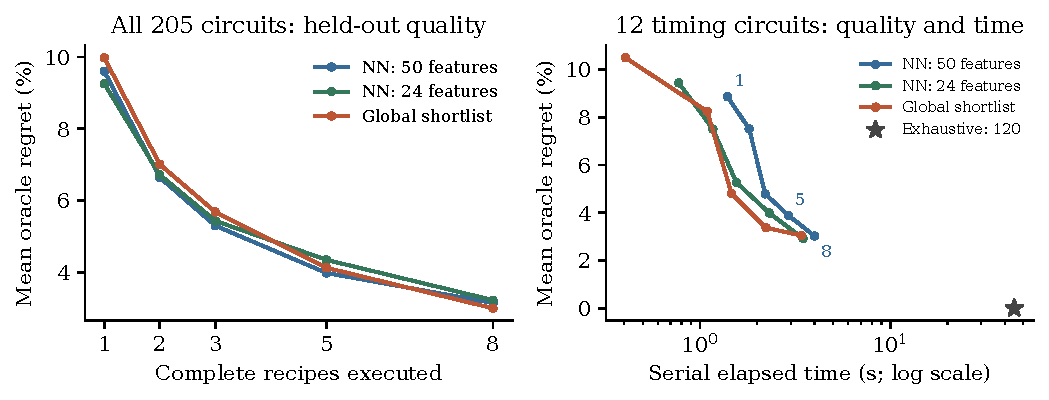
\includegraphics[width=\textwidth]{figures/neural_tradeoff.pdf}
\caption{Left: held-out quality over all 205 circuits as the candidate budget increases. Right: quality and fresh serial timing on the 12 timing circuits; blue labels give the full NN's recipe budget. The exhaustive reference evaluates all 120 candidates. The two panels use their stated circuit populations.}
\label{fig:nn-tradeoff}
\end{inlinefigure}

\subsection{Comparison with classical models}

Table~\ref{tab:main} reports the classical models on the same outer circuit folds. All learned selectors execute one complete recipe after feature collection. The adaptive selector chooses among the five classical model families inside the training partition. Its mean improvement is \PrimaryGain\, with interval \PrimaryCI; its mean regret is \PrimaryRegret. Its paired comparison with the fixed recipe gives $p=\PrimaryP$. Extra-Trees achieves a larger one-recipe mean gain than either NN variant in these experiments.

\begin{table}[htbp]
\centering\small
\begin{tabular}{@{}lrrrr@{}}
\toprule
\textbf{Selector} & \textbf{Gain (\%)} & \textbf{95\% interval} & \textbf{Regret (\%)} & \textbf{Win (\%)} \\
\midrule
Additive ridge & 0.12 & [-0.06, 0.31] & 9.81 & 20.5 \\
Interaction ridge & 0.02 & [-0.75, 0.78] & 9.74 & 47.8 \\
Extra-Trees & 1.11 & [0.60, 1.62] & 8.55 & 63.4 \\
Random Forest & 0.68 & [0.04, 1.28] & 9.06 & 56.6 \\
Gradient boosting & 0.45 & [-0.18, 1.02] & 9.29 & 56.6 \\
Adaptive selector & 0.73 & [0.25, 1.18] & 9.01 & 58.5 \\
Adaptive + margin gate & 0.72 & [0.24, 1.16] & 9.04 & 56.6 \\
Uniform random (expected) & -1.94 & [-2.53, -1.32] & 11.83 & -- \\
resyn2 & -0.02 & [-0.94, 0.86] & 9.66 & 51.2 \\
Best fixed training recipe & 0.00 & [0.00, 0.00] & 9.97 & 0.0 \\
Oracle (120 measured runs) & 8.61 & [7.90, 9.39] & 0.00 & 98.5 \\
\bottomrule
\end{tabular}

\caption{One-recipe selection at $\lambda=0.5$. Improvements are relative to the best fixed training recipe. Intervals bootstrap the 205 circuit averages after combining the three repeats. Win rates use those per-circuit averaged improvements.}
\label{tab:main}
\end{table}

The adaptive selector chose Random Forest in 7, Gradient boosting in 2, Additive ridge in 2, Interaction ridge in 2, Extra-Trees in 2 of the 15 outer folds. Its average improvement over \op{resyn2} was 0.36\%. After averaging the three test results for each circuit, it improved the fixed-recipe objective on 58.54\% of circuits and increased it on 35.61\%. Its mean within-circuit Spearman correlation was 0.268. The margin gate produced a mean gain of 0.72\% with interval [0.24\%, 1.16\%]. The confidence interval lies above zero, supporting an average gain on this circuit pool.


\begin{table}[htbp]
\centering\small
\begin{tabular}{@{}lrrr@{}}
\toprule
\textbf{Selector} & \textbf{Area gain (\%)} & \textbf{Delay gain (\%)} & \textbf{Both improve (\%)} \\
\midrule
Adaptive, one recipe & 0.54 & 0.54 & 26.8 \\
Adaptive, five recipes & 2.21 & 7.53 & 67.3 \\
Global, five recipes & 1.75 & 7.81 & 65.4 \\
resyn2 & -2.63 & 1.81 & 18.0 \\
\bottomrule
\end{tabular}

\caption{Individual area and delay improvements over the best fixed training recipe at $\lambda=0.5$. Positive gains mean reductions. Each metric is averaged within a circuit across repeats and then across the 205 circuits.}
\label{tab:components}
\end{table}

For the one-recipe adaptive selector, mean area improvement was 0.54\% and mean delay improvement was 0.54\% relative to the fixed recipe. Both improved on 26.83\% of circuits after combining repeats. With five verified recipes, the corresponding area and delay improvements were 2.21\% and 7.53\%. The weighted objective permits an area--delay trade-off, so these component measurements help interpret the combined gain.


\subsection{Which information helps?}

\begin{table}[htbp]
\centering\small
\begin{tabular}{@{}lrrr@{}}
\toprule
\textbf{Setting} & \textbf{Features} & \textbf{Gain (\%)} & \textbf{Regret (\%)} \\
\midrule
Full features; centered; full encoding & 194 & 0.81 & 8.86 \\
Static graph features & 168 & 0.00 & 9.76 \\
Static + mapping features & 172 & 0.21 & 9.47 \\
Probe features alone & 166 & 0.51 & 9.21 \\
Raw objective target & 194 & 0.77 & 8.87 \\
Within-circuit rank target & 194 & 1.13 & 8.42 \\
Operation-count encoding & 59 & 0.55 & 9.10 \\
Counts + position encoding & 143 & 0.29 & 9.42 \\
\bottomrule
\end{tabular}

\caption{Controlled boosting-model ablations at $\lambda=0.5$, evaluated on the same first five outer folds. Full features, full recipe encoding, and centered targets form the reference setting. Each row changes the stated component.}
\label{tab:ablations}
\end{table}

The full boosting configuration achieved 0.81\% mean gain in this repeat. Static graph features gave 0.00\%; adding mapping measurements gave 0.21\%; probe features alone gave 0.51\%. Using raw targets produced 0.77\% gain, and rank targets produced 1.13\%. Operation counts alone gave 0.55\% gain; the full sequence encoding gave 0.81\%.


\subsection{Transfer and candidate-library changes}

\begin{table}[htbp]
\centering\small
\begin{tabular}{@{}lrrrr@{}}
\toprule
\textbf{Test distribution} & \textbf{Circuits} & \textbf{Gain (\%)} & \textbf{95\% interval} & \textbf{Regret (\%)} \\
\midrule
MCNC to EPFL + ISCAS-85 & 26 & 1.61 & [-0.06, 3.31] & 8.75 \\
EPFL arithmetic held out & 7 & 0.95 & [-2.49, 4.91] & 8.72 \\
EPFL control held out & 9 & -2.69 & [-9.61, 3.16] & 15.77 \\
ISCAS-85 held out & 10 & 0.98 & [-0.35, 2.38] & 8.72 \\
MCNC held out & 179 & 0.00 & [0.00, 0.00] & 10.34 \\
\bottomrule
\end{tabular}

\caption{Adaptive one-recipe selection under changes in circuit distribution. Training and tuning use only circuits outside the stated test family or set. The MCNC-to-other split tests all 26 EPFL and ISCAS-85 circuits together.}
\label{tab:transfer}
\end{table}

Training on MCNC and testing on the other 26 circuits gave 1.61\% mean gain, with interval [-0.06\%, 3.31\%]. In the primary repeated protocol, family-specific mean gains were EPFL arithmetic 0.39\%; EPFL control 0.63\%; ISCAS-85 1.56\%; MCNC 0.70\%. The held-out arithmetic and control families contain seven and nine circuits, respectively, which gives their interval estimates a small sample base.


\begin{table}[htbp]
\centering\small
\begin{tabular}{@{}lrrr@{}}
\toprule
\textbf{Experiment} & \textbf{Gain (\%)} & \textbf{95\% interval} & \textbf{Regret (\%)} \\
\midrule
Delay objective & -0.79 & [-2.27, 0.70] & 18.61 \\
Area objective & -0.28 & [-1.05, 0.48] & 7.41 \\
30-recipe library & 0.36 & [-0.45, 1.15] & 6.91 \\
60-recipe library & 0.37 & [-0.59, 1.30] & 8.05 \\
25 training circuits & 0.19 & [-0.65, 1.09] & 9.30 \\
50 training circuits & 0.13 & [-0.73, 0.95] & 9.41 \\
100 training circuits & -0.62 & [-1.69, 0.37] & 9.69 \\
24 recipes unseen in training & 0.66 & [-0.28, 1.56] & 8.95 \\
\bottomrule
\end{tabular}

\caption{Boosting-model sensitivity experiments. Each objective weight and candidate library has its own training-only fixed-recipe comparator. Unseen-recipe training uses 96 candidates and evaluation offers all 120 candidates.}
\label{tab:sensitivity}
\end{table}

The area-only and delay-only experiments gave mean gains of -0.28\% and -0.79\%, respectively, with both confidence intervals including zero. Reserving 24 recipes from training gave 0.66\% mean gain with interval [-0.28\%, 1.56\%]. The average benefit in this unseen-recipe setting remains uncertain.


\section{Related Work}

Mishchenko, Chatterjee, and Brayton introduced scalable AIG rewriting with balancing and established the \op{resyn2} flow in ABC~\cite{mishchenko}. Their transformations form the vocabulary used in our recipes.

DRiLLS uses reinforcement learning to construct synthesis sequences and optimizes area under a timing constraint~\cite{drills}. FlowTune uses a domain-specific multi-armed bandit to explore synthesis flows~\cite{flowtune}. These approaches motivate selecting sequences that suit a particular circuit and accounting for the synthesis runs used during exploration.

OpenABC-D provides a large labeled synthesis dataset and supervised prediction tasks involving circuit graphs and recipe encodings~\cite{openabc}. We use a compact tabular representation and focus evaluation on the measured outcomes of selected recipes. Our dataset is generated from the selected benchmark sources using one mapping flow, which keeps the area and delay labels consistent across the pool.

\section{Reproducibility and Practical Use}

The release contains the final dataset, circuit inventory with source checksums, recipe library, ABC runner, feature extractor, nested evaluation code, fold assignments, out-of-fold predictions, result tables, figures, and a trained model artifact. ABC is pinned to commit \op{5d64f3b5}; the manifest records its full commit, benchmark commits, library checksum, dataset checksum, sampling seeds, and runtime. Appendix~\ref{app:repro} gives the environment and commands.

We compared all 12,300 overlapping pilot observations with our regenerated measurements. Area, delay, baseline measurements, and all graph and probe features agreed within numerical serialization precision. We independently repeated 24 sampled circuit--recipe pairs, six per source family. Their mapped area and delay reproduced exactly, and ABC established Boolean equivalence between each mapped result and its input circuit. For verification exports we remove external don't-care annotations, which describe input cases with no required output value, and compare the concrete Boolean networks. All 205 source-file checksums matched the saved inventory.


For a new combinational BLIF, BENCH, or AIGER circuit, the prediction command loads the saved NN, constructs its circuit features, and scores the recipe library. The full NN uses baseline mapping and probes. The graph-only NN skips the probes and uses graph statistics as inputs. With a verification budget, the command executes the selected shortlist and can write the best mapped circuit as a BLIF netlist. Its predicted score ranks candidates; the verified outputs provide measured area, delay, and the objective. The command also reports feature, prediction, verification, and model-load times.

\section{Discussion and Conclusion}

A small neural network can select from a fixed library of 120 synthesis recipes using measurements from earlier circuits. On 205 held-out benchmark circuits, executing one recommendation gave 0.19\% mean improvement over the best fixed training recipe, with interval [-0.40\%, 0.79\%]. This places its average objective near the fixed-recipe baseline. Executing five recommendations improved that baseline by 5.12\% and reduced mean regret to 3.99\%.

On the separate 12-circuit serial timing audit, one recommendation was 32.2 times faster than exhaustive search, and five recommendations were 15.4 times faster, including feature collection. The gain comes from replacing most full synthesis runs with a prediction. A global shortlist offers a similar quality--compute trade-off with less selection overhead, and Extra-Trees achieved a stronger one-recipe average improvement in the model comparison. These results make the budget explicit: a fixed recipe gives the cheapest decision, a short list gives better measured quality, and exhaustive evaluation gives the library optimum.


The pool contains 205 independent circuits, and 87\% come from MCNC. Family-transfer results therefore carry practical weight when considering a different design population. The labels describe one cell library and one synthesis timing setup. Larger circuits, sequential logic, other cell libraries, and physical implementation require additional measurements.

\begin{thebibliography}{9}\small
\bibitem{abc} Berkeley Logic Synthesis and Verification Group. ABC: A System for Sequential Synthesis and Verification. \url{https://github.com/berkeley-abc/abc}.
\bibitem{mishchenko} A. Mishchenko, S. Chatterjee, and R. Brayton. DAG-Aware AIG Rewriting: A Fresh Look at Combinational Logic Synthesis. In \emph{DAC}, pp. 532--535, 2006. \url{https://doi.org/10.1145/1146909.1147048}.
\bibitem{epfl} L. Amar\`u, P.-E. Gaillardon, and G. De Micheli. The EPFL Combinational Benchmark Suite. In \emph{IWLS}, 2015. Benchmark repository: \url{https://github.com/lsils/benchmarks}.
\bibitem{hdl} ISP RAS. hdl-benchmarks: Collection of Digital Hardware Modules and Projects. \url{https://github.com/ispras/hdl-benchmarks}.
\bibitem{nangate} The OpenROAD Project. NanGate45 Platform and Typical-Corner Open Cell Library. \url{https://github.com/The-OpenROAD-Project/OpenROAD-flow-scripts/tree/master/flow/platforms/nangate45}.
\bibitem{drills} A. Hosny, S. Hashemi, M. Shalan, and S. Reda. DRiLLS: Deep Reinforcement Learning for Logic Synthesis. In \emph{ASP-DAC}, pp. 581--586, 2020. \url{https://arxiv.org/abs/1911.04021}.
\bibitem{flowtune} W. Lau Neto, Y. Li, P.-E. Gaillardon, and C. Yu. FlowTune: End-to-End Automatic Logic Optimization Exploration via Domain-Specific Multi-Armed Bandit. \emph{IEEE Transactions on Computer-Aided Design of Integrated Circuits and Systems}, 2022. \url{https://arxiv.org/abs/2202.07721}.
\bibitem{openabc} A. B. Chowdhury, B. Tan, R. Karri, and S. Garg. OpenABC-D: A Large-Scale Dataset for Machine Learning Guided Integrated Circuit Synthesis. arXiv:2110.11292, 2021. \url{https://arxiv.org/abs/2110.11292}.
\end{thebibliography}

\appendix
\section{Complete Structural Feature Definitions}
\label{app:features}

Let $I$ be the input count, $O$ the output count, $N$ the AND-node count, and $L$ the graph depth. An edge into an AND node is a \emph{fanin}; edges leaving a signal contribute to its fanout. A node's level is one plus the larger level of its two input signals, with input signals at level zero.

\small
\begin{longtable}{@{}p{4.1cm}p{10.2cm}@{}}
\toprule
\textbf{Feature or group} & \textbf{Definition and interpretation}\\
\midrule
Inputs, outputs, AND nodes, depth (4) & $I$, $O$, $N$, $L$. Interface dimensions, amount of logic, and longest logical path.\\
Edges (1) & $2N+O$, including each AND node's two inputs and output connections.\\
Size ratios (4) & $N/L$, $(2N+O)/(N+I)$, $I/N$, and $O/N$. Describe logic density relative to paths and interface size.\\
Fanout statistics (5) & Mean, maximum, and standard deviation over input and AND nodes; fraction with fanout above one; mean over AND nodes alone. Higher fanout indicates signal reuse or branching.\\
Complemented-edge fraction (1) & Fraction of AND fanin edges carrying an inverted signal.\\
Level-width statistics (4) & Maximum and mean number of AND nodes per level, width standard deviation divided by its mean, and maximum width divided by $N$. Describe how logic is distributed across depth.\\
Fanin-level imbalance (3) & Mean and maximum absolute level difference between an AND node's two input signals, and the fraction of nodes with a difference of at least two.\\
XOR-pattern fraction (1) & Fraction of AND nodes matching a local three-node exclusive-OR or exclusive-NOR construction. This is a structural pattern count.\\
Local reconvergence fraction (1) & Fraction of AND nodes whose two input neighborhoods share a nonconstant signal within one predecessor step. This describes nearby paths that diverge and meet again.\\
\bottomrule
\end{longtable}
\normalsize

The ten log-transformed static columns are input count, output count, AND count, depth, edge count, nodes per depth, maximum fanout, maximum width, mean width, and maximum fanin-level difference. Ratios and fractions retain their original scale.

\section{Environment and Reproduction}
\label{app:repro}

\begingroup\small
\begin{tabular}{@{}ll@{}}
\toprule
\textbf{Item} & \textbf{Recorded value} \\
\midrule
Processor allocation & 8 logical CPUs; synthesis sweep: 5 workers \\
Python & 3.12.3 \\
numpy & 1.26.4 \\
pandas & 3.0.2 \\
scipy & 1.17.1 \\
scikit-learn & 1.8.0 \\
lightgbm & 4.6.0 \\
matplotlib & 3.6.3 \\
joblib & 1.5.3 \\
torch & 2.11.0 \\
ABC commit & \texttt{5d64f3b5f3bb9db6f3d77636a65e99ba3ee9d799} \\
Library SHA-256 & \texttt{8d540a4d4cf6d09d27c87ad0\ldots} \\
Cross-validation seeds & 0, 1, 2; inner split seed: outer fit seed + 1000 \\
Sampling seeds & Pilot recipes: 7; extension: 17; subset: 23; unseen recipes: 29 \\
Bootstrap & 2,000 circuit resamples; seed 2026 \\
\bottomrule
\end{tabular}

\endgroup

From the project root, the main commands are:
\begin{verbatim}
python3 -m pip install -e .
python3 scripts/fetch_sources.py
make -C tools/abc -j4 ABC_USE_NO_READLINE=1
circuit-recipe sweep --workers 5
python3 scripts/run_experiments.py
python3 scripts/run_neural.py
python3 scripts/benchmark_neural_runtime.py
python3 scripts/report.py
circuit-recipe train
python3 scripts/build_paper.py
\end{verbatim}

The supplied dataset allows the learning and reporting stages to run directly. The source download and sweep commands regenerate the synthesis measurements. Checkpoints preserve completed circuits during a resumed sweep.

For example, to verify three model-ranked recipes on a new circuit and save the best mapped result:
\begin{verbatim}
circuit-recipe select design.blif --verify 3 --netlist out.blif
\end{verbatim}

\end{document}
